%----------------------------------------------------------------------------
\chapter{Mérőrendszer fejlesztése}
\label{sec:Fejleszt}
%----------------------------------------------------------------------------


A felszedő adapteren alkalmazott elektromos készülékekhez $12$~V egyenfeszültség van alkalmazva, így az egyik fő követelménye a fejlesztendő rendszernek, hogy ezen a feszültségen működjön. A korábban már említett por- és olajszennyezés, valamint a kompaktság és modularitás is fontos, hogy szem előtt maradjon. A rendszer kialakításában nagy szerepet játszik még a biztonságtechnikai megfontolás, valamint a meglévő kialakításra való ráillesztés, a támogató mérnöki munka lecsökkentése. A \ref{felszedo_adapter} ábrán látható a felszedő adapter, amelyre a mérőrendszer tervezése készült.
\begin{figure}
	\centering
	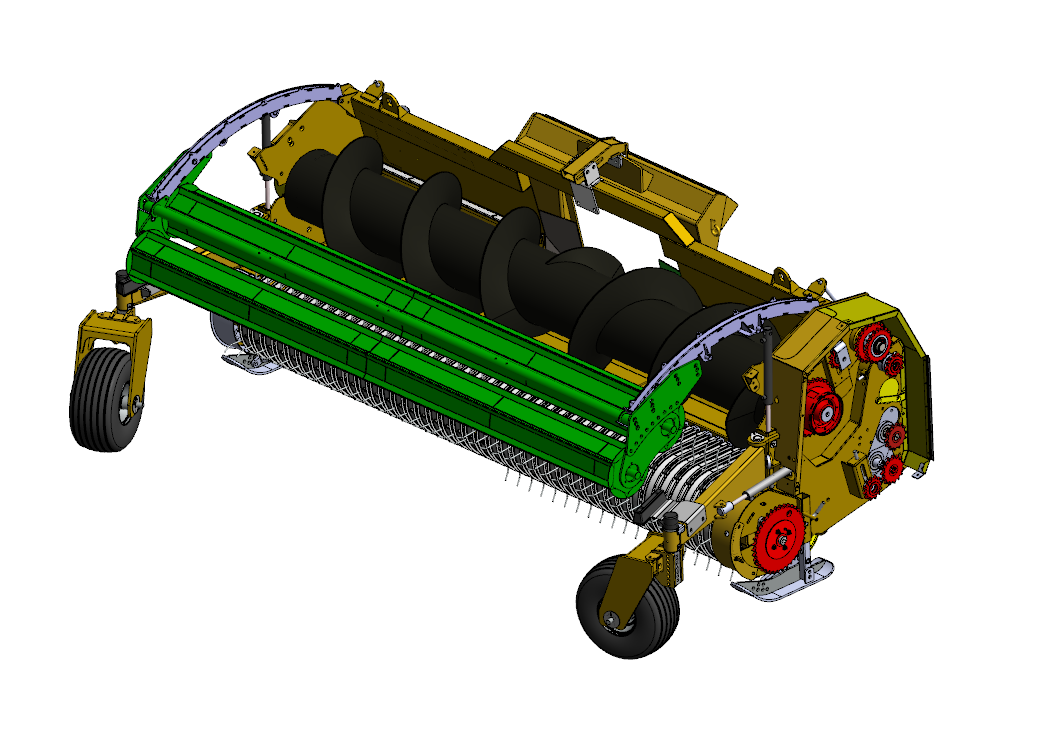
\includegraphics[width=\columnwidth*5/10]{figures/egesz_adapter.png}
	\caption{Felszedő adapter CAD modellje.}
	\label{felszedo_adapter}
\end{figure}

%----------------------------------------------------------------------------
\section{Szenzorok}
%----------------------------------------------------------------------------

A feladat során három szenzor alkalmazása szükséges, melyek mind fordulatszámot mérnek, azonban különböző céllal és kialakításban. Az első cél a nyomatékhatároló be- és kimeneti oldali tengelyeinek összehasonlítás, amelyhez két fordulatszámmérő szenzor alkalmazása szükséges. Ezen felül a fogakkal ellátott felszedő tengely fordulatszámának mérése is a feladat része, ez azonban a visszajelzésben tájékoztató jellegű, biztonságtechnikai feladata nincs. A mérendő tengelyek elhelyezkedése látszik a \ref{merendo_tengelyek} ábrán, ahol a feketével színezett tengely a csiga, az ezüstre színezett pedig a fogas felszedő tengelye.
\begin{figure}
	\centering
	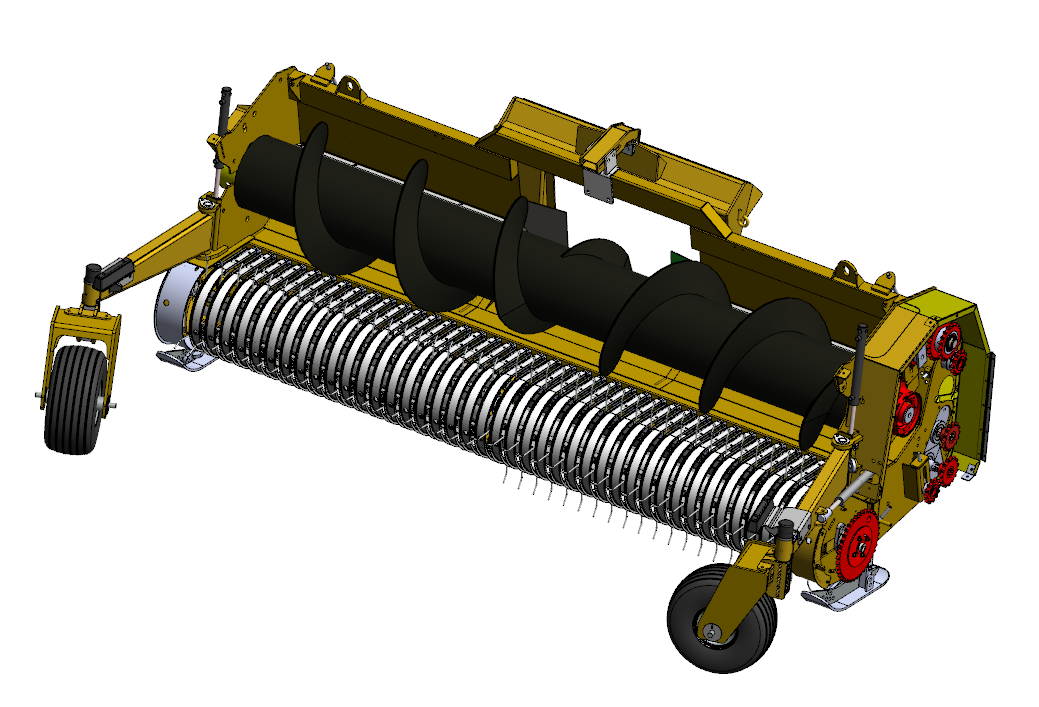
\includegraphics[width=\columnwidth*6/10]{figures/merendo_tengelyek.png}
	\caption{Mérendő tengelyek CAD modellje.}
	\label{merendo_tengelyek}
\end{figure}

A nyomatékhatároló a \ref{nyomatekhatarolo} ábrán figyelhető meg -- a felszedő tengely lánckerekével együtt --, ahol a külső, szélesebb tengely a bemeneti oldal, amit a silózóból érkező nyomaték lánchajtáson keresztül meghajt, valamint a belső tengely, a takarmány összeterelésére alkalmazott csiga tengelye pedig a kimeneti oldal. A meghajtás oldalán a tengely hozzáférhető, ugyanis ez borítja a csiga tengelyét. Itt van lehetőségünk akár a tengely, akár a fogas tárcsa mérésére, amely a fogaslánc hajtását adja tovább. Azonban a csiga tengelyéhez való hozzáférés limitált, valamint a tengely meghosszabbítása sem lehetséges, mivel a burkolattól biztonságos távolságban már lehet kihúzni akár egy tárcsát vagy mérendő tengelyt. Ezért a csiga tengelyének másik végét szükséges mérni, ahol egy lemez vagy tárcsa felhelyezésének lehetősége is megvan, ezt a \ref{tuloldali_csiga} ábra mutatja. A felszedő tengelye egy lánckerékben végződik, amely megfelelhet, a tengely helyett akár, egy mérési felületnek.
\begin{figure}
	\centering
	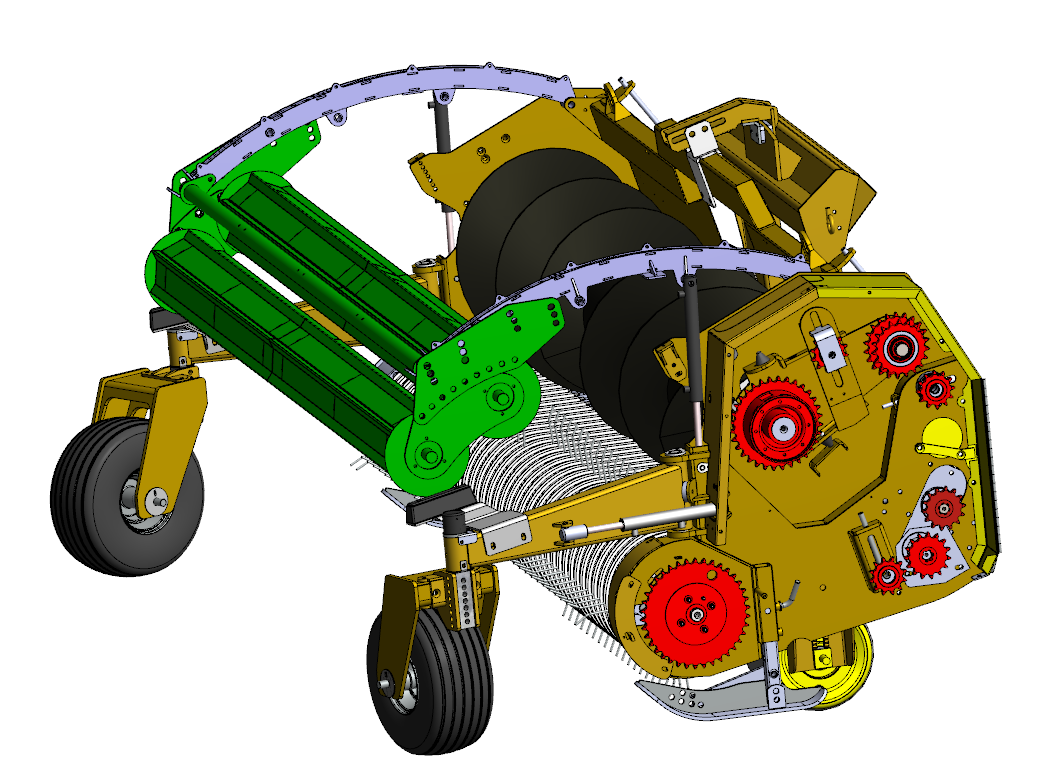
\includegraphics[width=.7\columnwidth]{figures/hajtas_oldal.png}
	\caption{A nyomatékhatároló, és hajtás felőli oldalon látható mérendő tengelyek (piros lánckerekek).}
	\label{nyomatekhatarolo}
\end{figure}
\begin{figure}
	\centering
	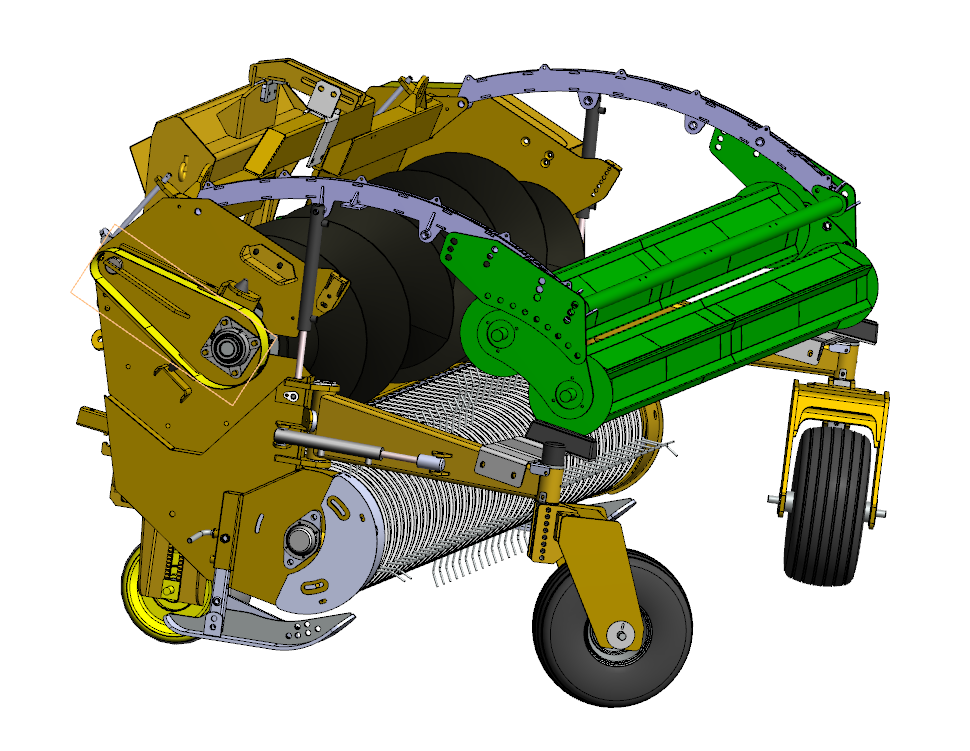
\includegraphics[width=.7\columnwidth]{figures/csiga_oldal.png}
	\caption{A csiga tengelyének mérési helye (szürke tengelyvégződés).}
	\label{tuloldali_csiga}
\end{figure}

%----------------------------------------------------------------------------
\subsection{Szenzorválasztás}
%----------------------------------------------------------------------------

A \ref{szenzorok_szakirodalom} fejezetben feltárt mérési elvek, szenzorok közül a következő kritériumok segítik a döntést leszűkíteni:

\textbf{Por- és olajállóság}: a szenzor élettartamát nem befolyásolhatják ezek a szennyező anyagok, valamint szennyezett környezetben a mérés pontosságát meg kell tartania. Az első kritériumnak a legtöbb ipari kialakítású szenzor megfelel, hiszen megfelelő ház, burkolat védi őket a külvilágtól. A második kritérium kizárja a szenzorok nagy hányadát, ugyanis ezáltal a levegőn keresztül közlendő fizikai jelek továbbítása és (a lerakódó rétegek által) olvasásának minősége jelentős mértékben romlik, valamint az összes mérés, amely során fizikai kontaktus szükséges problémákba ütközhet, mint a felületek súrlódása során sérülés, vagy a súrlódási együttható növekedésével járó hőtermelődés. Ezáltal kizárhatjuk a következő mérési elveket: 
\begin{itemize}
	\item \textbf{Lineáris és helikális potenciométer}, hiszen kontaktusra alapszik mindkettő szenzor.
	\item \textbf{Kapacitív elven alapuló szenzorok}, a közeg vezetőképességének változása bizonytalan méréshez vezetne.
	\item \textbf{Optikai elven működő szenzorok}, a levegő és a felszíni szennyeződés is rontja a mérést.
	\item \textbf{Ultrahang szenzorok}, a közvetítő közeg nem alkalmas a fizikai hullámok terjedésének állandóságához.
	\item \textbf{Radarok}, amelyek szintén hang alapján működnek, így nem megfelelőek.
	\item \textbf{Elektromos vezetővel kódolt tárcsa}, a szénkefék kontaktusa nem alkalmas a felgyülemlő szennyeződések mellett.
	\item \textbf{Stroboszkópos szenzorok}, szintén optikai elven alapulnak.
\end{itemize}

\textbf{Geometriai megfontolások}: A mérendő tengelyek esetében nincs, vagy nagyon minimális tér van a burkolatig, így a kiegészítő tengely vagy tárcsa, illetve szenzorok tengelyirányú szerelésére nincs lehetőség. Az érzékelők beépítését, a kiegészítő mérnöki feladatok mellett, a kábelezés és biztonságtechnikai megfontolások is bonyolítják. A csiga tengely meghajtással szembeni tengelyen van lehetőség ilyen segédalkatrészek kialakítására, azonban az érzékelési elv esetében érdemes egyforma szenzorokra törekedni, könnyű összehasonlíthatóság kialakítása végett. Így tehát a tengelybe épített, vagy annak kiegészítésével alkalmazható szenzorokat szintén elvethetjük:
\begin{itemize}
	\item \textbf{Kódolt tárcsák}
	\item \textbf{Rezolver és Szinkró}, a forgórész beépítése szükséges lenne.
	\item \textbf{Sebesség- és elfordulásmérő giroszkópok}, a forgástengelyben helyezkednek el.
	\item \textbf{Analóg tachométerek}, analóg és digitális kialakításukban is egy tekercset szükséges építeni a tengelybe.
	\item \textbf{Szöggyorsulásmérők}, a tengelyben helyezkednek el.
	\item \textbf{Induktoszin}, a sín felszerelése elengedhetetlen.
\end{itemize}

\subsubsection{Alkalmas mérési elvek}

Az alkalmas szenzorok mind a induktív mérési elven alapulnak az előző szekcióban említett okok miatt. A \ref{szenzorok_szakirodalom} fejezetben tárgyalt technológiák közül az induktív távolságmérésre alkalmas fizikai jelenségek (elektromágneses indukció, örvényáramok, Hall-effektus), és azokat alkalmazó szenzorok (LVDT/RVDT, induktív, mágneses tachométerek) maradtak. További szűkítésre a \ref{celkituzes} fejezetben tárgyalt támogató fejlesztés elkerülése végett, ahol lehetséges ott lánckerék mérése optimális, vagyis a hajtás oldali szenzoroknál. Az egyforma és egyszerű kialakításhoz egy fogas lemez alkalmazásával a csiga túloldali tengelyét is mérni tudjuk ugyanazon szenzor felhasználásával. 

\subsubsection{Szenzor kialakítása}

A kiválasztott technológiák után, a választást a kialakítás és költségek limitálják. Alapvetően az élettartam megnövelése --a szennyező környezetben -- érdekében, mindenképpen egy ipari kialakítású szenzorra van szükség. Ezen belül is egy $12$~V feszültséggel kell működjön, valamint a \ref{celkituzes} fejezetben említett modularitás végett az ipari szenzorok között megtalálható csatlakozós kialakítás alkalmazása ideális, amelyek kábelei cserélhetőek, hiszen így a kábel és a szenzor egymástól függetlenül kicserélhető, akár javítható.

Ilyen kialakítású szenzorok esetén, a Hall-érzékelős fordulatszámmérők a piacon kevésbé jellemzők, feltehetőleg a bonyolultságuk és ezáltal költségességük végett. Az induktív távolságmérő azonban egy elterjedt szenzor, amellyel egy jelen alkalmazás fordulatszámmérésére a lehető legalkalmasabb. 

\subsubsection{Szenzor paraméterei}

A szenzor választásakor egyes paramétereknek a környezeti kialakításnak kell megfelelniük. 
\begin{itemize}
	\item \textbf{Beszerelési átmérő}: A lánckerék (16B1 típusú) fogainak vastagsága (modulja) $16$~mm, amelynél keskenyebb vastagságú kell legyen a szenzor a fals jelek elkerülése érdekében. A túl keskeny kialakítás a mérési távolságot limitálja, így az optimális választás az M12-es menetes $12$~mm beszerelési átmérőjű szenzorház lesz a jelen alkalmazásra.
	\item \textbf{Kapcsolási távolság}: A mérendő tárcsáknak a radiális ütése (a kerület menti eltérése a tervezett átmérőtől) általában $0,3-0,4$~mm, ez megengedné a szenzorok közel állítását, azonban a lánckeréken lerakódott zsír és por elkerülése érdekében érdemes nagyobb távolságból mérni. A lemezből készült fogazott tárcsán a gyártási pontosság $\pm0,5$~mm, a szerelési illesztésekből még hozzáadható $\pm0,5$~mm, így ennek a kerületi ütése nagyjából $\pm1$~mm lesz. Mindkét esetben a mérési távolság, a biztonságra való tekintettel, legalább $4$~mm ajánlott.
	\item \textbf{Mérési frekvencia}: Az a frekvencia, amellyel a szenzor mérési eredményeket rögzít. A mérendő mennyiség változásának frekvenciájának kétszeresét (Nyquist frekvencia) szükséges meghaladnia mérési frekvenciának, a mérés megbízhatóságának érdekében \cite{Morris2016d}. A nyomatékhatároló lánckerekén $z=32$ a fogszám, a működési fordulatszáma $180-250$~1/perc körül mozog, azonban a meghajtás megengedi a $350$~1/perc elérését is, így erre érdemes tervezni biztonsági megfontolásokból. Ezen tengely túloldalán való mérés azonos fordulatszámmal dolgozik, a fogszám azonban tetszőleges lehet, így a lánckerék fogszámánál mindenképp kisebbre ajánlott tervezni, legegyszerűbb esetben a fogszám $z=1$. A felszedő tengely fordulatszáma jóval alacsonyabb, $85-150$~1/perc tartományban mozog, azonban ennek a lánckeréknek a fogszáma $z=38$. A szükséges mérési frekvencia a maximális fordulatszám másodpercenként, így frekvenciát adva és a fogszám szorzatának kétszerese lesz, mivel a fogszám a jel csúcsainak számát adja meg. Ez alapján a \ref{frek_nyom} és \ref{frek_felsz} egyenletekből származó jel olvasásához szükséges frekvenciák közül a nagyobb az elvárt mérési frekvencia: $\approxeq375$~Hz.
\end{itemize}
\begin{equation}
	f_{nyomatékhatároló}'=\frac{350}{60}\cdot32\cdot2=373.33\text{Hz}
	\label{frek_nyom}
\end{equation}
\begin{equation}
	f_{felszedő}'=\frac{150}{60}\cdot38\cdot2=190\text{Hz}
	\label{frek_felsz}
\end{equation}

\subsubsection{Választott szenzor}

A követelmények megfelelő szenzornak Datalogic IS-12-H1-S2 induktív szenzor rövid verzióját választottam, amely M12-es csatlakozóval és beszerelési vastagsággal, $8$~mm kapcsolási távolsággal, amelynek mérési frekvenciája $500$~Hz, így bőven meghaladja a követelményt \cite{datalogic_catalog}. A szenzor a beszerelési felületre merőlegesen végzi a mérést, a forgás tengelyével szintén derékszöget zár be, ezáltal a tárcsa vagy kerék fogainak mérésére képes. Ez a szenzor analóg feszültségjelet továbbít, az érzékelt test távolságának függvényében, amelyt egy három erezetű kábel egyik szálán továbbítanak, ahol a másik két erezet pedig a tápfeszültség és földelés. A \ref{kabelezes_1} és \ref{kabelezes_2} ábrák mindkét irányból vázlatszerűen mutatják a három szenzorból érkező kábelek elvezetését, amelyek a (jelen modellben nem ábrázolt) pneumatikus és egyéb kábelek útját követik, valamint az adatfeldolgozó helyét jelző dobozt, amelyek a tápfeszültség és az analóg jeleket továbbítják. Ehhez három darab egyenként legalább hat méter hosszú, 3 erezetű M12-es csatlakozóval rendelkező kábelt ajánlanék.
\begin{figure}
	\centering
	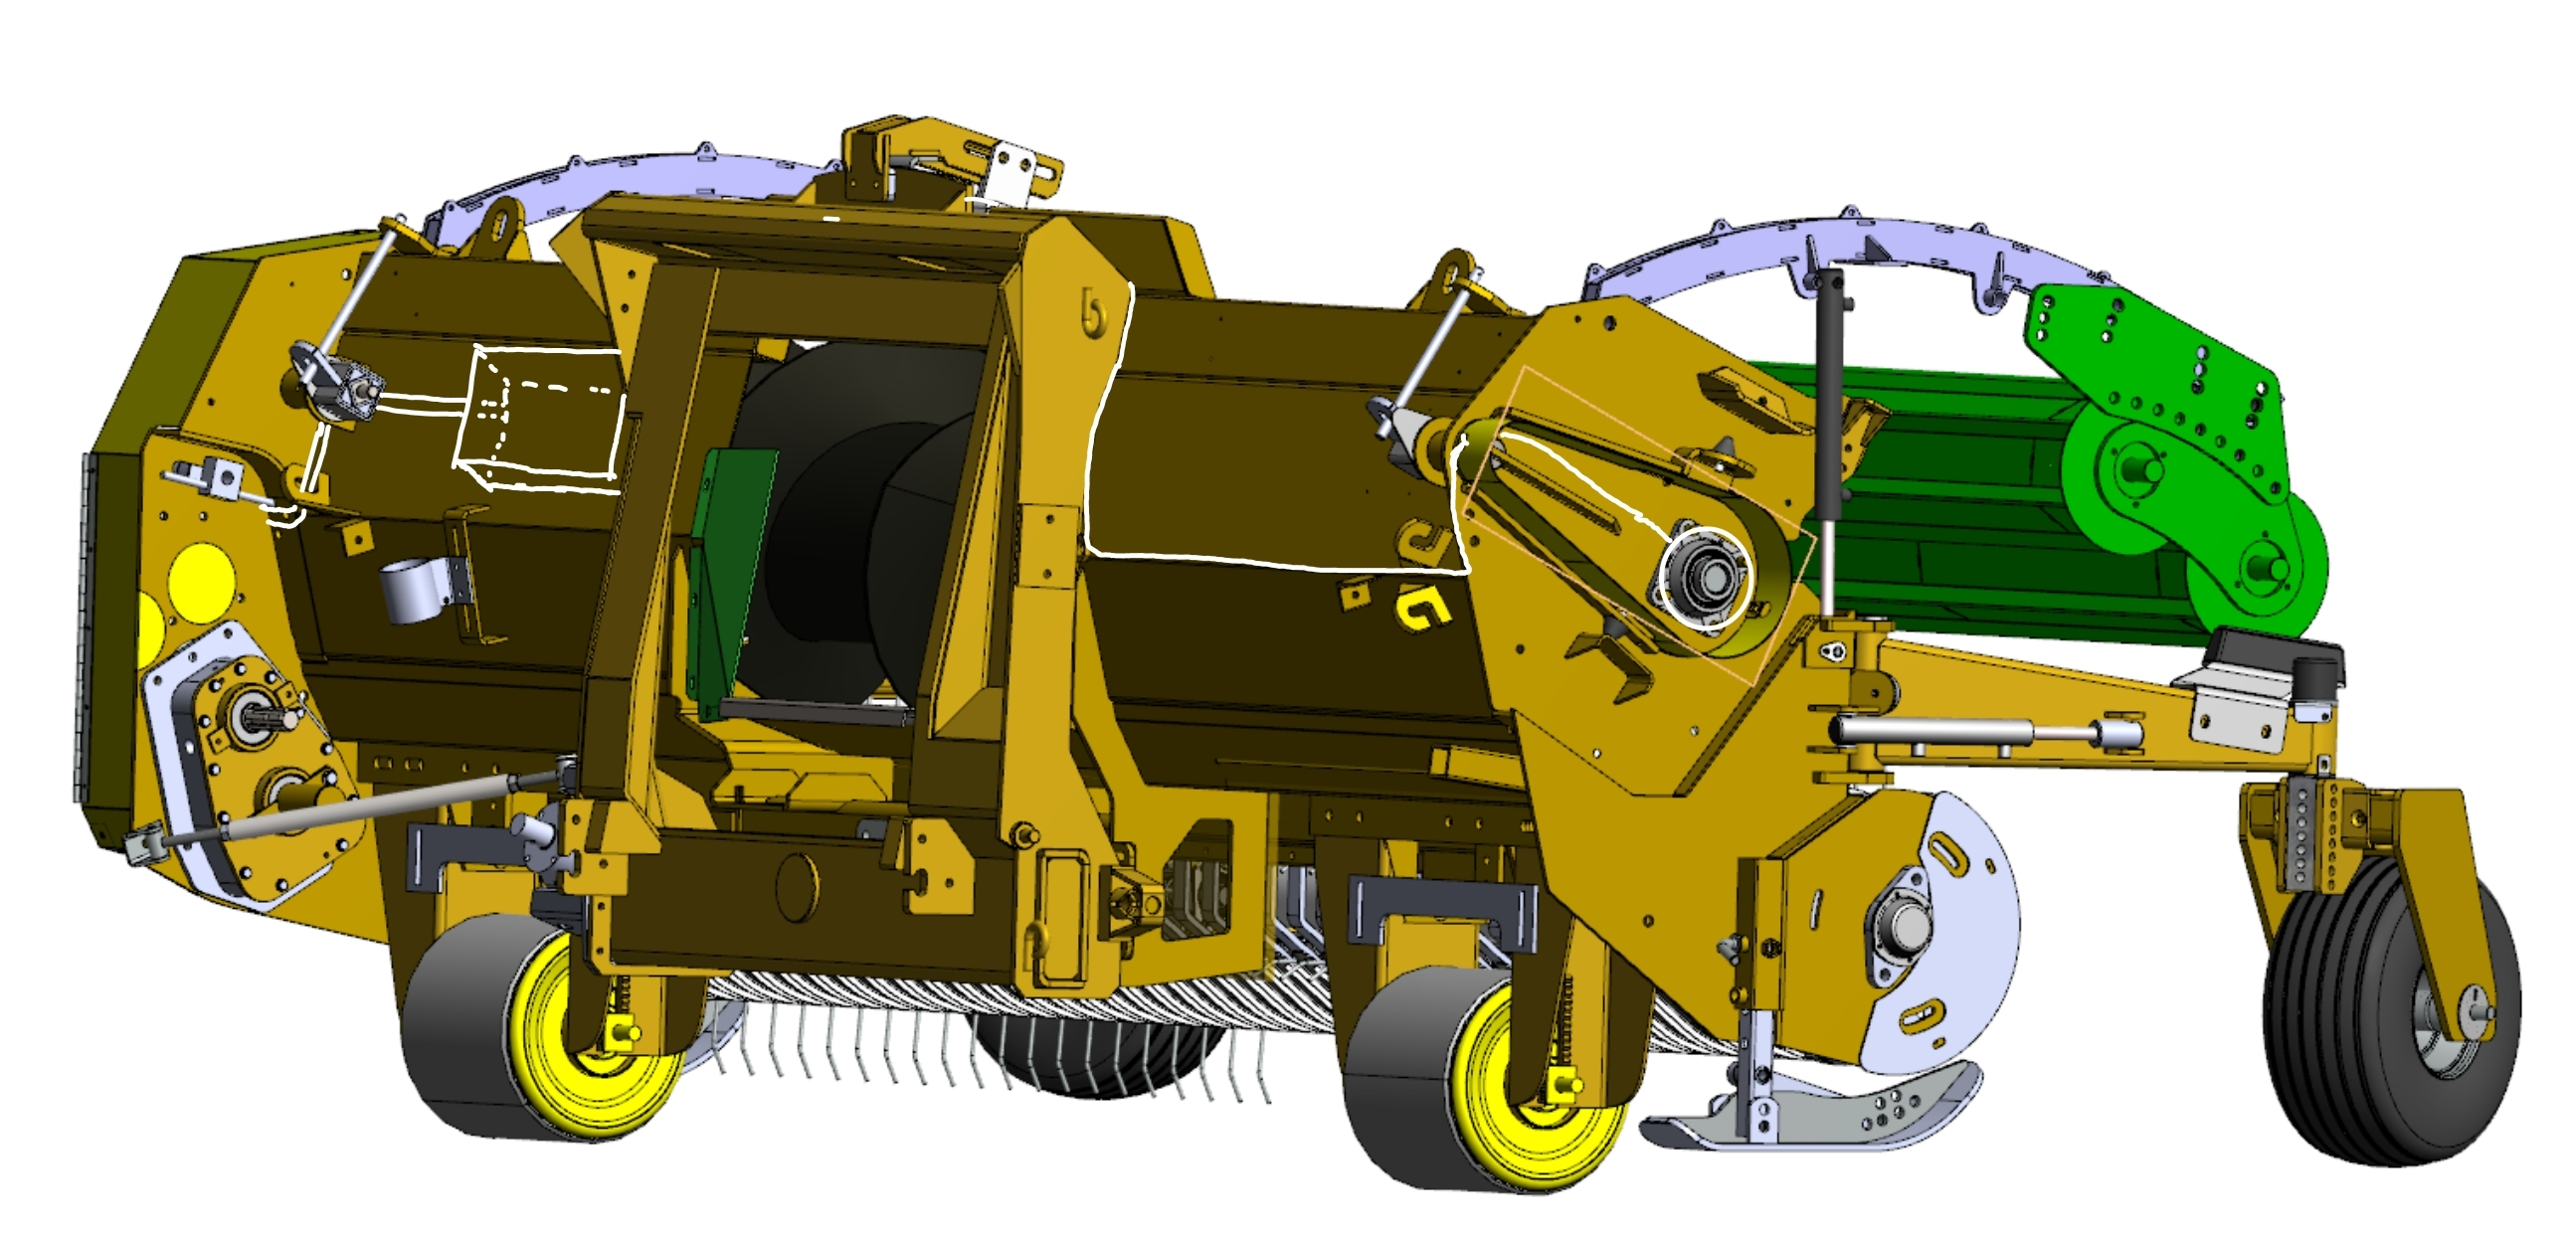
\includegraphics[width=\columnwidth*6/10]{figures/rajzolt_kabelezes_1.jpg}
	\caption{Kábel elvezetésének vázlata a meghajtás oldala felől}
	\label{kabelezes_1}
\end{figure}
\begin{figure}
	\centering
	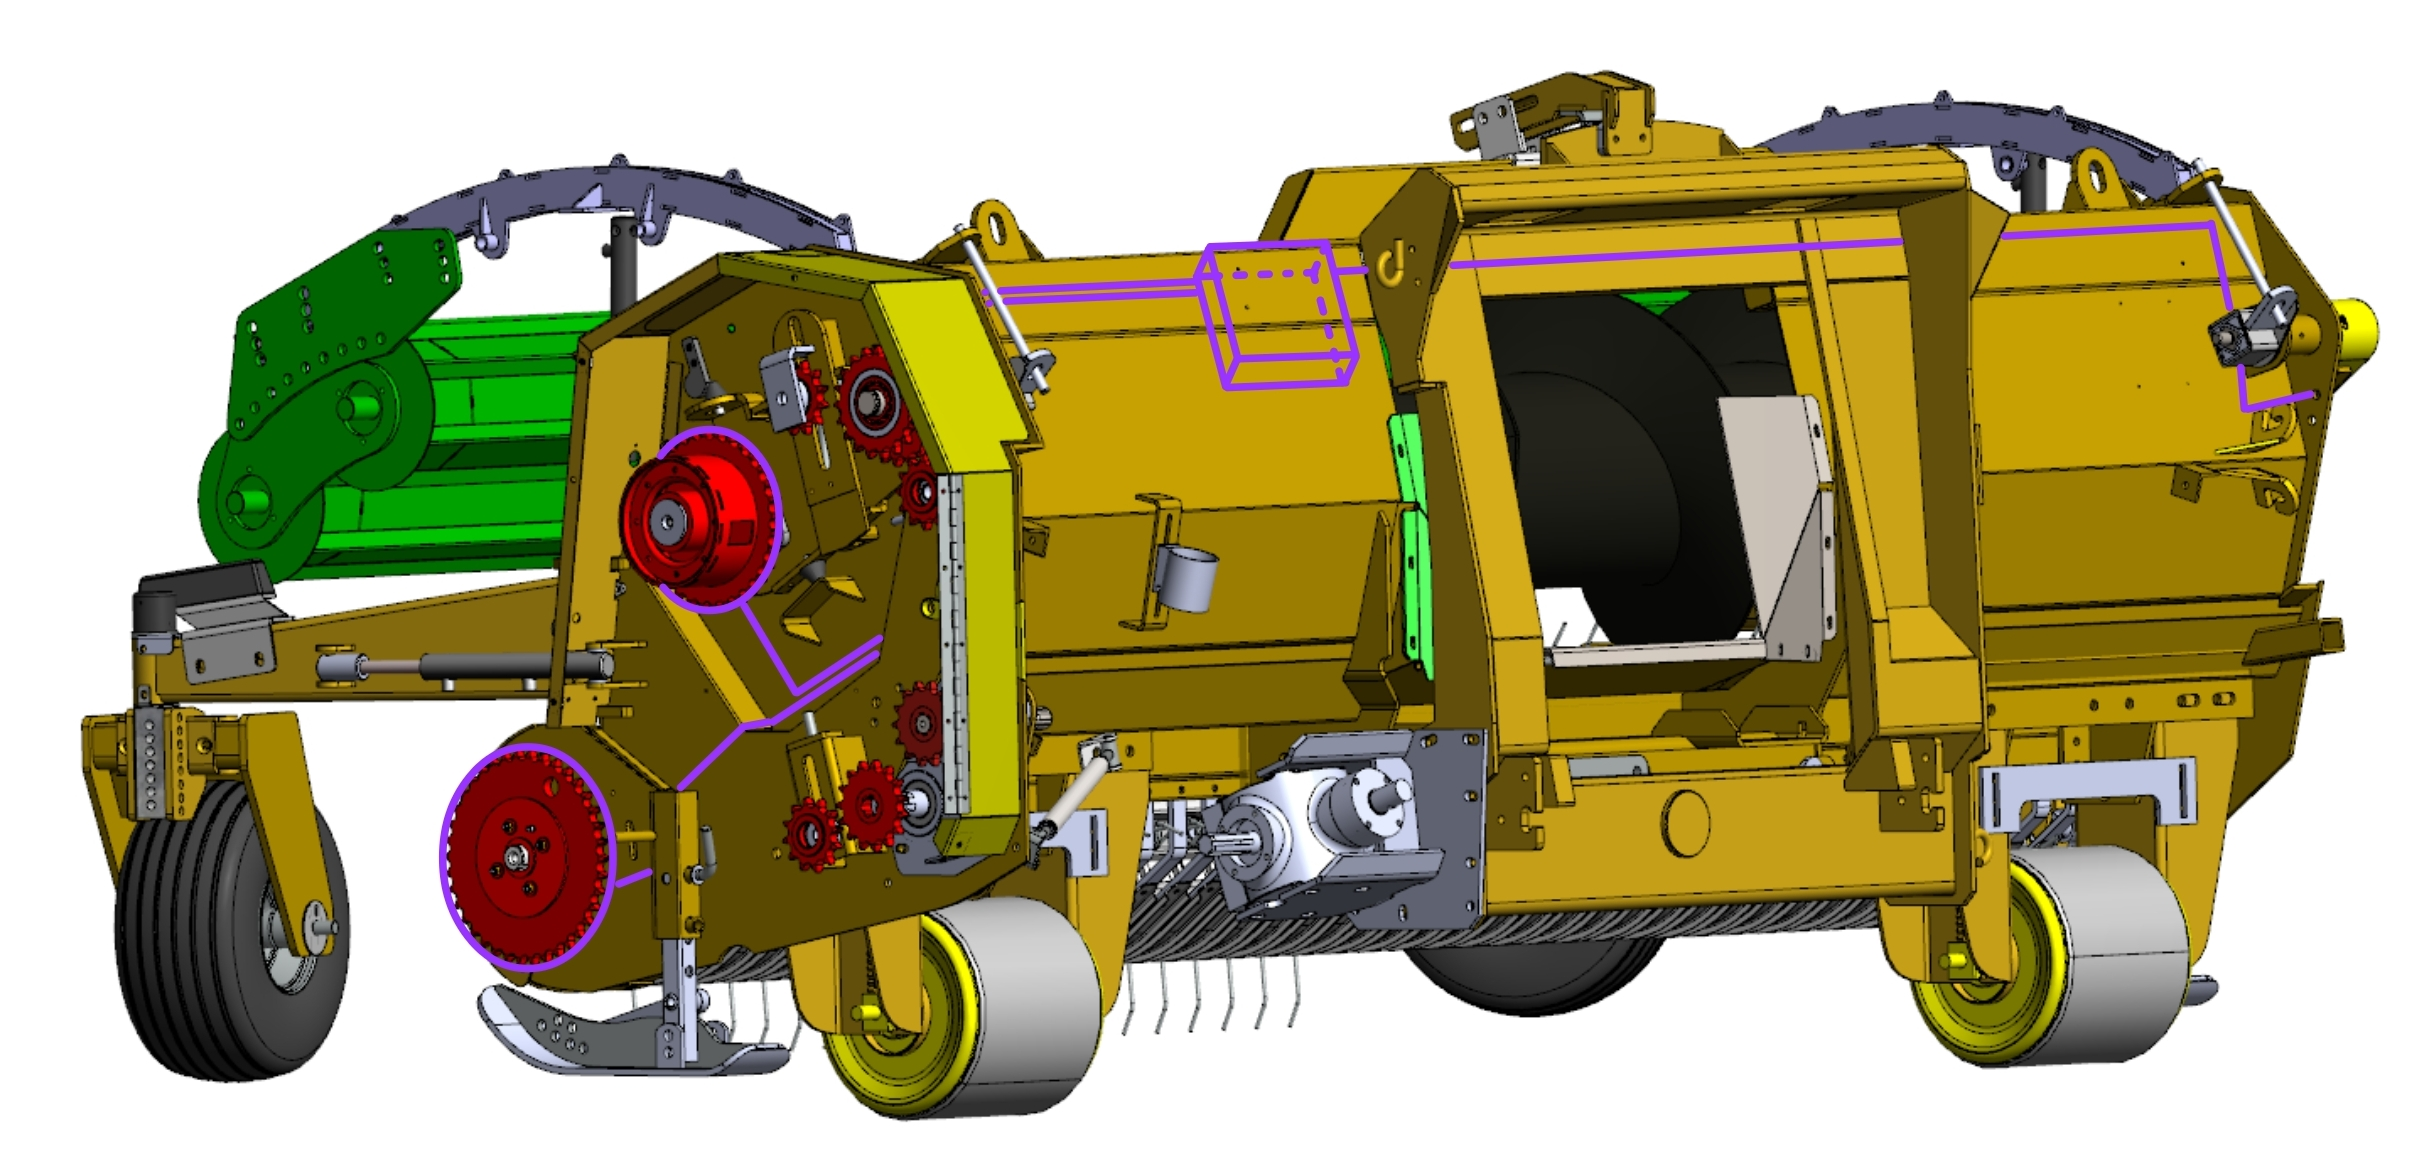
\includegraphics[width=\columnwidth*6/10]{figures/rajzolt_kabelezes_2.jpg}
	\caption{Kábel elvezetésének vázlata a csiga mérésének oldala felől}
	\label{kabelezes_2}
\end{figure}

%----------------------------------------------------------------------------
\subsection{Jelek}
\label{jelek}
%----------------------------------------------------------------------------

A beérkező feszültség jelek változása a fogak elhaladását követi le, így a fogak megjelenéséhez tartozó feszültség tartományt lehet felhasználni irányadóként. A különböző szenzorok nekik megfelelő feszültségértékekkel, valamint fogszámokkal rendelkeznek. Így a fordulatszám számítása mérési pontonként eltér, de a számítási mód megegyezik, ez pedig a \ref{ford_alt} egyenletben szemléltetett, ahol $n$ a fordulatszám, $z_1$ az elhaladt fogak száma, $z_{tárcsa}$ az adott tárcsának a fogszáma, $t$ pedig az eltelt idő percben, mivel a fordulatszám 1/perc vagy rpm. Például ha egy perc a vizsgált időintervallum, és ha a lemeznél a fogszám $z_{tárcsa}=1$, akkor az abban a percben megszámolható fog elhaladások, megegyeznek a fordulatszámmal: $n = \frac{z_1}{60}$~rpm.
\begin{equation}
	n = \frac{z_1}{z_{tárcsa}\cdot t}
	\label{ford_alt}
\end{equation}
Ezáltal lesz összehasonlítható két szenzorból érkező jel, valamint ez jeleníthető meg a fordulatszámként a kezelőfelületen.

%----------------------------------------------------------------------------
\section{Visszajelzés}
\label{visszajelz}
%----------------------------------------------------------------------------

A visszajelzés feladata, hogy az ember-gép kapcsolatot megvalósítsa. A jelzés biztonságtechnikai szerepe akkor merül fel, ha a nyomatékhatároló két oldalán lévő fordulatszám eltér egymástól, és ezáltal a nyomatékhatárolónak, vagy az adapternek rongálásához vezetne a gép tovább üzemelése. Ennek a megoldásaira több opció is rendelkezésre áll. Az alapvető megközelítés egy fény villogása, vagy folyamatos világítása az adapteren, a vezetőfülkéből jól látható helyen és magasságban. A fényjelzés mellé gyakori a hangjelzés, amely a fülkén belül hasznos lenne, azonban a zajos környezetben, ahogyan egy silózó operál, nem célravezető. A silózóval való kommunikáció azonban ennek a dolgozatnak a látószögén kívül esett, ugyanis a silózók számos gyártója különböző szabványokat használ az adapterrel való kommunikációra, valamint a silózók kialakítása is eltér, és ezekhez az információkhoz való hozzáférés körülményes. Ezt megkerülő opció a vezeték nélküli csatlakozás a rendszerhez. Erre több protokoll is alkalmas, viszont ehhez a megfelelő szabályozó eszköz szükséges, amely a következő (\ref{szabalyozas}) fejezetben lesz tárgyalva, hiszen az határozza meg a legtöbb paraméterét a visszajelző rendszernek is.

\subsection{Visszajelzés eszközei}

A fény visszajelzésére egy $12$~V feszültségen működő, víz- és porálló, napsütésben is megfelelő fényerejű, valamint cserélhető alkatrész szükséges. Ennek mind eleget tesznek az ipari visszajelzőlámpák, amelyek robusztusok és $12$~V-os kivitelben is megtalálhatóak. A választás a Barthelme LED jelzőfényére esett \cite{barthelme_led}, amely $22$~mm beszerelési átmérővel rendelkezik, a jelzőfény átmérője pedig $29$~mm. Az ipari környezetben a figyelemfelkeltésre, veszély jelzésére gyakran a piros jelzőfényt alkalmazzák, így azt választottam. A felszerelése egy furatba helyezés után csavaros rögzítéssel van ellátva, valamint a csatlakozói kábelek bekötésére alkalmasak, így könnyen cserélhető ez az eszköz. Az előlap IP65 (Ingress Protection) védettséggel rendelkezik, amely a por behatolásával szemben teljes védelem (6) és vízsugarak elleni védelmet (5) jelenti, így megfelel az alkalmazásnak. A fény felhelyezése a szabályozó rendszer védődobozára kerül felhelyezésre, hiszen ez látható, szintén IP védett, és meg is egyszerűsíti a kábelezését, hiszen nem kell elvezetni és hosszú kábelt alkalmazni.

%----------------------------------------------------------------------------
\section{Vezérlés}
\label{szabalyozas}
%----------------------------------------------------------------------------

Jelen alkalmazás egy irányítási feladat, ugyanis a bemenetek nem közvetlenül a kimenet és a referencia különbségéből következnek. A vezérlő eszközök első sorban az előző fejezetben kidolgozott szenzorok jeleit fogadják be, és az adatfeldolgozást végzik el. További feladatuk, hogy a visszajelző rendszert üzemeltessék, a jel kiadását, a kommunikációt megvalósítsák. 

%----------------------------------------------------------------------------
\subsection{Vezérlés eszközei}
%----------------------------------------------------------------------------

Az irányítási eszközök esetében a $12$~V feszültség valójában egy meghatározó paraméter. Ugyanis a korábbi eszközök kiválasztásánál léteznek változatok, amelyek ugyanazon eszköz $12$~V-on való működtetését megengedik, azonban a szabályozó eszközöknél ez kevésbé jellemző. A feszültség konvertálása egy külső eszközzel lehetséges, azonban az egyszerűség és átláthatóság, valamint a könnyebb cserélhetőség végett, inkább egy önmagában $12$~V feszültségen működő rendszer választása vonzóbb. A rendszernek a három szenzor analóg bemenetét, valamint a visszajelzőfény egy digitális kimenetét kell tudnia kezelni. Ezen felül a vezeték nélküli kommunikáció kezelése is szükséges.

\subsubsection{Eszközválasztás}

A PLC rendszerek szokványosan $24$~V tápfeszültséggel működnek, habár akadnak $12$~V-os modellek, a gyártók nem feltétlen fektetnek rájuk hangsúlyt. Ezen felül a PLC a legköltségesebb, legtöbb modulra felosztott berendezés, a nagyobb rendszerek kivitelezésére van kialakítva.

A mikrovezérlők általában $3,33$ és $5$~V közötti egyenfeszültségen üzemelnek, az áramkörök védelme egy külön feladat, a PLC és relé kialakításokhoz képest, amelyek általában IP védettek. A programozás rugalmassága sem feltétlen szükséges, hiszen a grafikus, logikára alapozott nyelvek is rendelkeznek a jelen alkalmazás kivitelezéséhez szükséges eszközkészlettel.

A programozható relék esetén gyakori a $12$~V-os változat, habár széles . Az alacsony ki- és bemenetek száma nem okoz problémát, hiszen a három analóg bemenet és egy digitális kimenet számainak eleget tesz. A PLC-khez hasonlóan IP védettségük megfelelő, és programozásuk szintén Létra Diagram (LD) és Funkcióblokk Diagram (FBD) alapú. A programozható relék között több megoldás is van az internetes, felhő alapú a vezérlőmodulok, amelyek akár szerverek futtatására, és adattárolásra is képesek. A \ref{prog_rele} táblázat bemutatja az egyes modelleket, amelyek alkalmasak jelen felhasználásra. A táblázatban a DI: digitális bemenet (digital input), AI: analóg bemenet (analog), DO: digitális kimenet (digital output), az AO pedig az analóg kimenet (analog output) jelenti.
\begin{table}[]
	\renewcommand{\arraystretch}{1.4}
	\scalebox{0.73}{
		\begin{tabular}{|l||l|l|l|l|}
			\hline
			& \begin{tabular}[c]{@{}l@{}}Schneider Electric\\ Zelio Logic \cite{zelio_adatlap}\end{tabular} & IDEC SmartRelay \cite{idec_adatlap} & Siemens LOGO! 8\cite{siemens_logo_adatlap} & Eaton Easy \cite{eaton_easy_adatlap} \\ \hhline{|=||=|=|=|=|}
			Modellszám           & SR2B121JD                                                                & FL1F-B12RCE                                                 & 6ED1052-2MD08-0BA2                                                     & EASY-E4-UC-12RCX1                                                                     \\ \hline
			Feszültség           & 12V                                                                      & 12/24V                                                      & 12/24V                                                                 & 12/24V                                                                                \\ \hline
			Bemenetek            & 4 DI + 4 AI                                                              & 4 DI + 2 AI                                                 & 4 DI + 4 DI/AI                                                         & 4 DI + 4 DI/AI                                                                        \\ \hline
			Kimenetek            & 4 DO                                                                     & 8 DO                                                        & 4 DO                                                                   & 4 DO                                                                                  \\ \hline
			Számítási frekvencia & 1 kHz                                                                    & 5 kHZ                                                       & 5 kHz                                                                  & 5 kHz                                                                                 \\ \hline
			Kommunikáció         & N/A                                                                      & N/A                                                         & Modbus TCP                                                             & MODBUS TCP/IP                                                                         \\ \hline
			Program felület      & \begin{tabular}[c]{@{}l@{}}ZelioSoft 2\\ (LD, FBD)\end{tabular}          & \begin{tabular}[c]{@{}l@{}}WingLGC\\ (LD, FBD)\end{tabular} & \begin{tabular}[c]{@{}l@{}}LOGO! Soft Comfort\\ (LD, FBD)\end{tabular} & \begin{tabular}[c]{@{}l@{}}EASYSOFT-SWLIC/easySoft7\\ (EDP, LD, FBD, ST)\end{tabular} \\ \hline
			Internet csatlakozó  & Nincs                                                                    & Ethernet RJ45                                               & Ethernet RJ45                                                          & Ethernet RJ45                                                                         \\ \hline
			SD memory            & Nincs                                                                    & MicroSD                                                     & MicroSD                                                                & Nincs                                                                                 \\ \hline
			Méret                & 90x68x10                                                                 & 90x71,5x58                                                  & 90x71,5x58                                                             & 90x72x58                                                                              \\ \hline
			Hozzávetőleges Költség (Ft) & 75 000                                        & 69 000                 & 58 000                                                      & 72 000\\ \hline
		\end{tabular}
	}
	\caption{$12$~V-os programozható relék összehasonlítása}
	\label{prog_rele}
	\renewcommand{\arraystretch}{1}
\end{table}

Ezeket szem előtt tartván a SIEMENS LOGO! 6ED1052-2MD08-0BA2 vezérlő/logikai modulját ajánlanám \cite{siemens_logo_adatlap}, amely nem csak internet hozzáféréssel rendelkezik, de akár MicroSD-ről is felprogramozható, valamint az adattárolásra is alkalmazható. Megfelelőek a paraméterei, valamint egy megbízható gyártó modellje, így a támogatás és a szoftver minősége bizonyosan nem szenved hiányt, ezen felül a költsége is kedvező.

Az internetes kommunikáció akkor jöhet létre, ha az eszköz az RJ45 csatlakozóaljzaton keresztül kapcsolódik az internetre, ugyanis önmagában vezeték nélküli csatlakozásra nem képes. A SIEMENS által gyártot kommunikációs modul (6GK7142-7EX00-0AX0), amely LTE hálózathoz képes csatlakozni amelyhez SIM-kártyát képes befogadni, nagyjából a vezérlőegység háromszorosát teszi ki költségében, mivel számos protokoll és további I/O lehetőségeket is kínál. Kizárólag a Wi-Fi kapcsolat végett ennek a beszerelését nem ajánlanám. Erre a célra lehetséges egy router, vagy repeatert alkalmazni, amelyek jóval kedvezőbb áron a jelen alkalmazásban, ugyanazt a funkciót ellátják. Erre $12$~V-os rendszert nem találtam, amely kis mérettel is rendelkezik, az általam ítélt legjobb megoldás a a GL-iNet által forgalmazott GL-AR300M16 vezeték nélküli mini router \cite{router}, amely $5$~V-os feszültségen működik, micro USB csatlakozón keresztül. A router képes repeater-ként működni, amelyhez egy RJ45 csatlakozó is rendelkezésre áll, amelyen keresztül internetet tud szolgáltatni a relének, egy vezeték nélküli hálózat jelenlétében. A feszültség átalakítónak egy sok helyen fellelhető $12$~V - $5$~V átalakítót javasolnék, amelynek micro USB kialakítású kimenete van \cite{fesz_atalak}.
%----------------------------------------------------------------------------
\subsection{Programozás}
%----------------------------------------------------------------------------

A vezérlőegység felprogramozása a LOGO! Soft Comfort elnevezésű szoftverben történik, amely a SIEMENS által fejlesztett Létra Diagram és Funkcióblokk Diagram nyelveket alkalmazó környezet. Ezek a nyelvek alapvető tudást igényelnek, azonban könnyen tanulható, grafikai felületen elkészíthető, előre megírt függvények, számlálók, késleltetések és logikai elemek alkalmazásával programozható. Amennyiben az internethez kapcsolódik a relé, a felprogramozás azon keresztül is végezhető, alternatíva egy SD kártyára exportált kód is behelyezhető a berendezésbe. 

%----------------------------------------------------------------------------
\subsection{Adatfeldolgozás}
%----------------------------------------------------------------------------
Az algoritmus feladata, hogy a \ref{jelek} fejezetben tárgyalt fordulatszámot előállítsa. A programban ehhez késleltetéseket, és számlálókat szükséges használni, amelyek egy változó -- Létra Diagramban tekercs által reprezentált -- értékét tudják megváltoztatni, például $0,1$~másodperc letelte alatt összegyűlt jel alapján számolható az összes fordulatszám üzem közben, és ezeknek az összehasonlítása után nullázható az összes változó, a számítás újrakezdhető. A webfelületen megjelenített adatok akár ezeket a végértékeket írhatják ki, a megadott időközönként frissülve. A nyomatékhatároló és csiga fordulatszámának összehasonlítása során a két változó különbségét kell egy bizonyos határértéknél alacsonyabbnak ítélni, hiszen a szenzorok és a mérés eredendően kis mértékű bizonytalanságokkal van terhelve egy ilyen környezetben. A további hibák eltűrése végett, a határérték átlépésével nem egyből adunk hibajelet, hanem csak pár másodperc elteltével folyamatosan jelenlévő eltérés fennmaradása esetén. Ennek oka, a bizonytalanságon kívül, hogy a nyomatékhatároló egy adott időn belül még nem sérül, csak hosszabb megcsúszási intervallumon, így nem szükséges minden tized másodperc megcsúszásának jelzése. Ezek a számok, és időintervallumok csak a tapasztalati visszajelzésekből, kísérletezésekből tudjuk pontosan meghatározni, így ezeket nem tudom jelen dolgozatban megadni.

%----------------------------------------------------------------------------
\subsection{Elhelyezés}
%----------------------------------------------------------------------------

A irányítási rendszer, vagyis a relé és a jelzőfény, illetve ezekhet tartozó, valamint a szenzoroktól jövő táp- és adatkábelekhez egy IP védett doboz felhasználását ajánlanám. A doboznak két alkatrészt kell tartalmaznia, valamint a külsejére szerelhetőnek kell lennie a harmadiknak. A programozható relé dimenziói: $90$x$71,5$x$58$~mm, a router mérete: $58$x$58$x$25$~mm, a jelzőfény átmérője pedig $22$~mm, a beszerelés után pedig $37$~mm hosszú a dobozban található része. Így a kényelmes elrendezés végett üres teret hagyva a dobozt legalább $200$x$100$x$80$~mm-re méretezném. Az elérhető IP65-ös, szabványos kötődobozok közül a $200$x$155$x$80$~mm-es méret ennek megfelelő. A dobozból kijövő kábelek esetén pedig az egyszerűség és szerelhetőség végett tömszelence beszerelése lenne a választásom. A doboz elhelyezése az adapter silózó felőli oldalának fenti részén, a \ref{doboz_elhelyezes} ábrán kijelölt helyen lenne ideális.
\begin{figure}
	\centering
	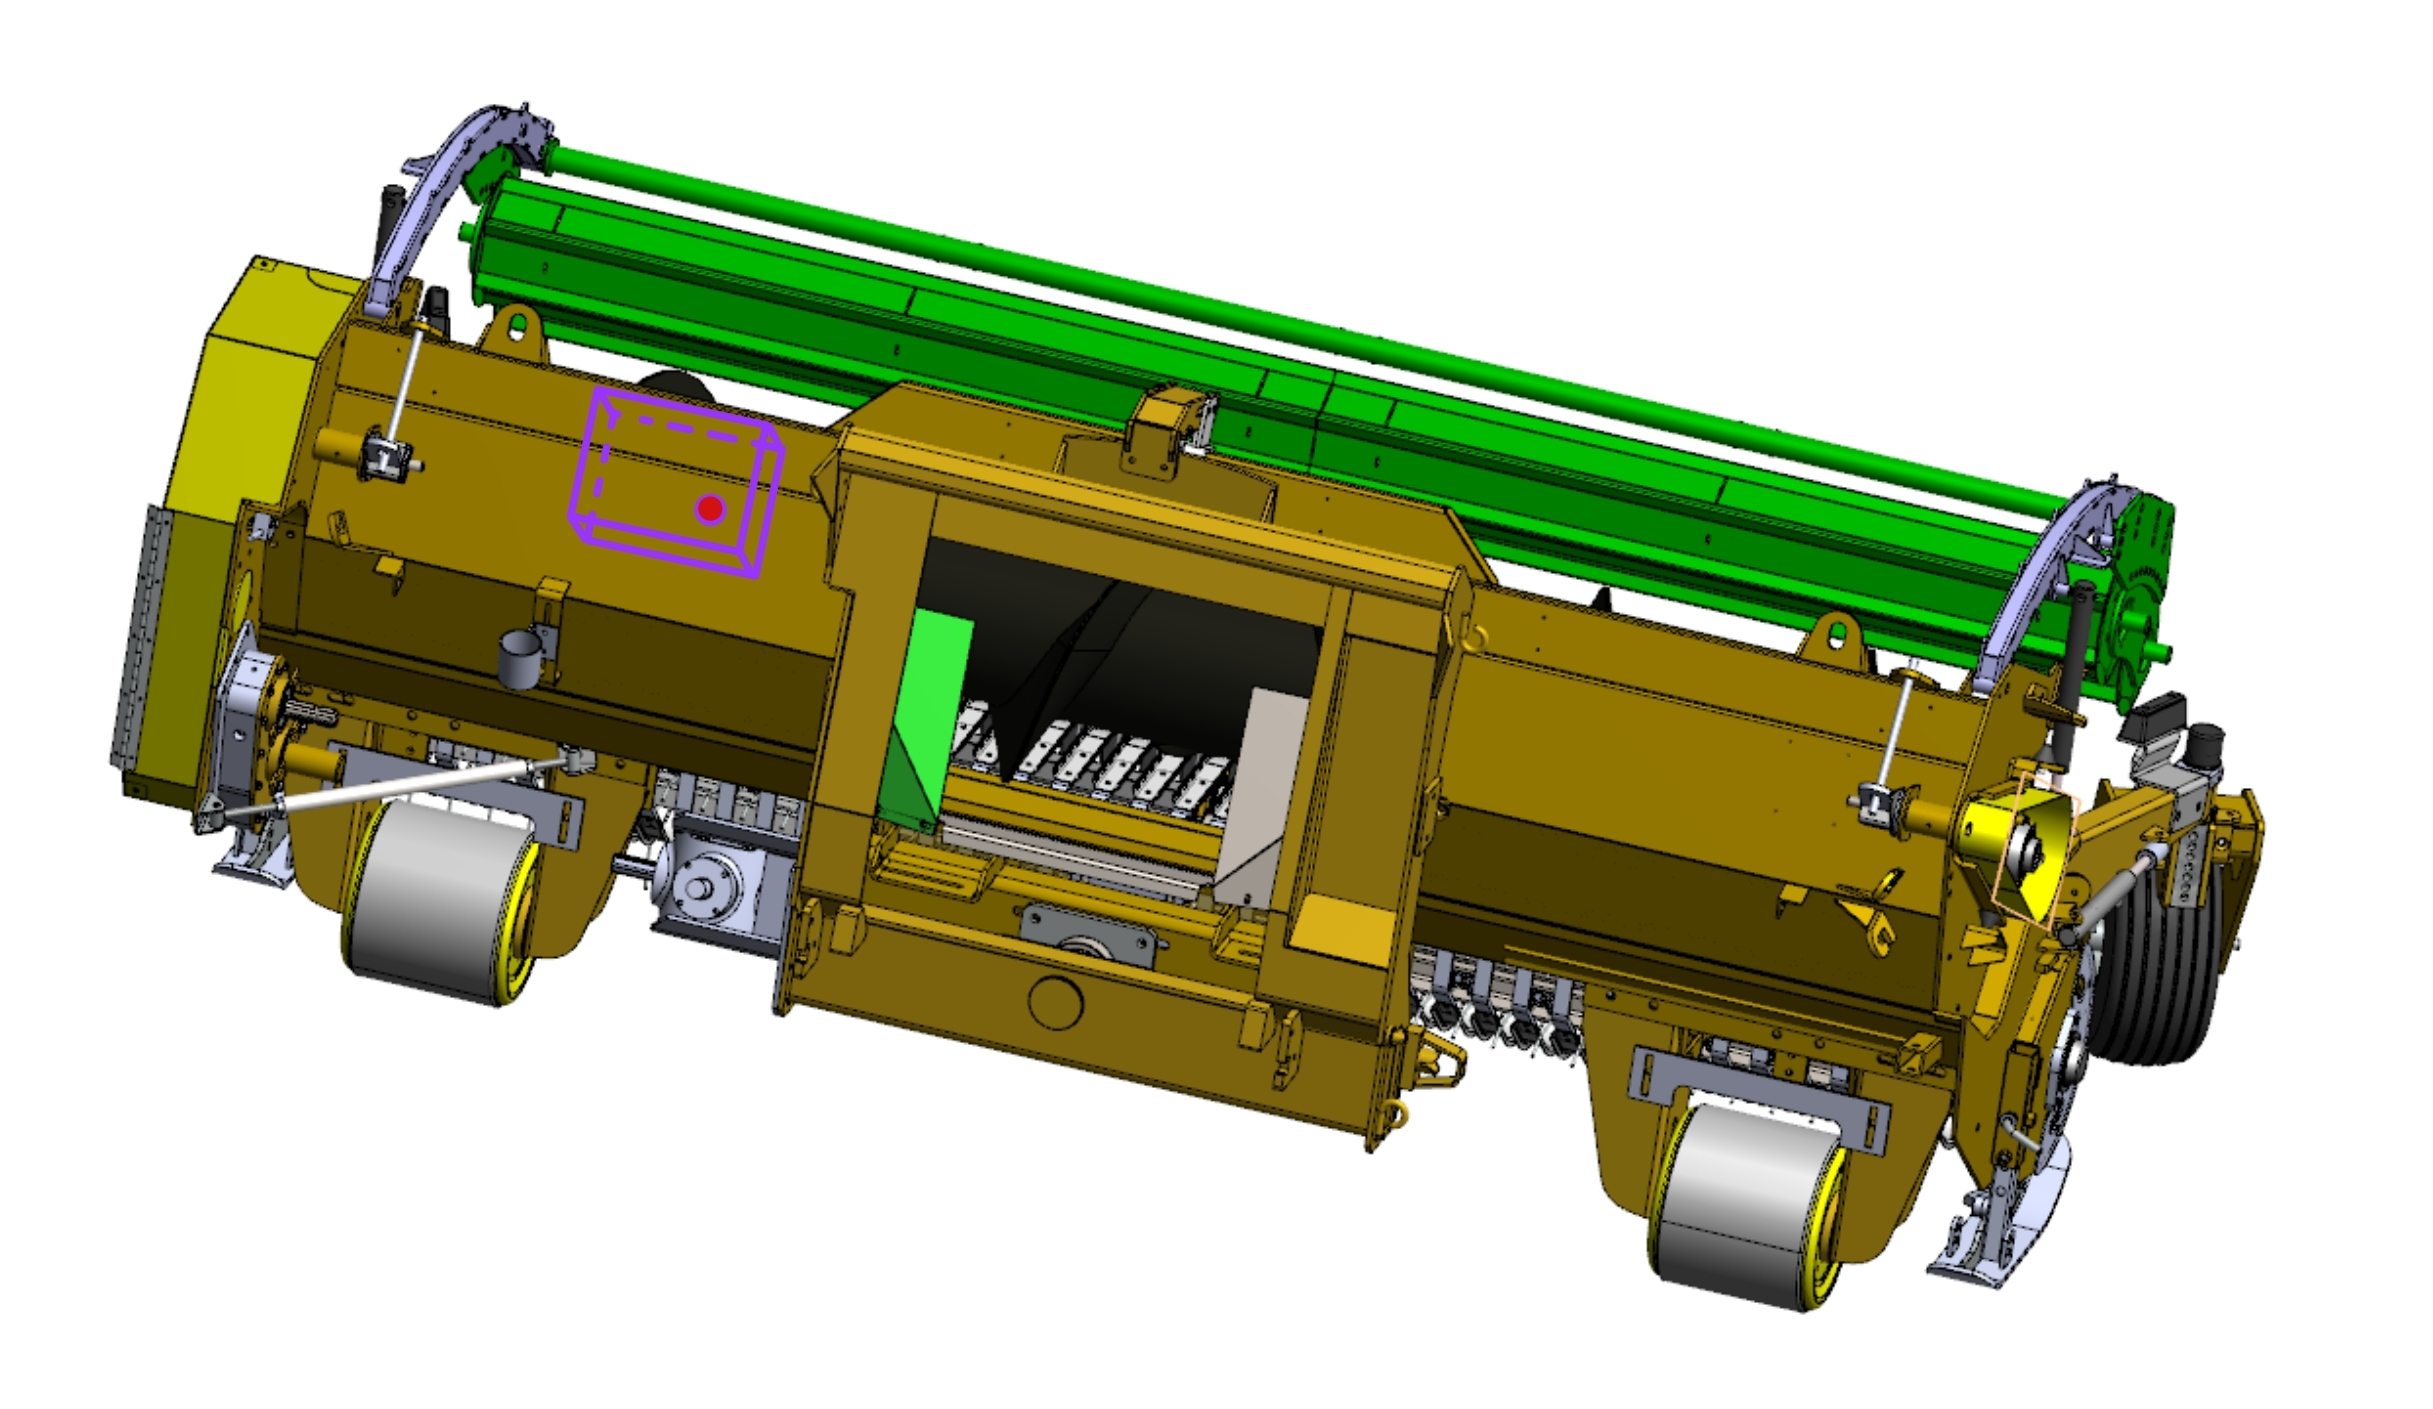
\includegraphics[width=\columnwidth*7/10]{figures/rajzolt_doboz.jpg}
	\caption{Doboz elhelyezésének vázlata}
	\label{doboz_elhelyezes}
\end{figure}

%----------------------------------------------------------------------------
\section{Alkalmazási lehetőségek}
%----------------------------------------------------------------------------

A rendszer kézenfekvő alkalmazása a Hevesgép Kft. megfelelő adapterein való üzembiztonsági és diagnosztikai feladatok elvégzése. Azonban a rendszer általános architektúrája, a programozható relé rendszer, a visszajelzés, és esetleg a szenzorok más projektek alapját is képezhetik, ahol hasonló mérési feladatok kerülnek. A szenzorok alkalmazása kétes más helyzetekben, ugyanis ha nincs lehetőség egy tárcsa vagy lánckerék mérésére, minden bizonnyal egy alternatív szenzor választása szükséges, amelyben segítségként akár a dolgozatot is lehet felhasználni.
%----------------------------------------------------------------------------
\subsection{Üzembiztonsági megoldások}
%----------------------------------------------------------------------------

A fejlesztett rendszer alapvető feladata, hogy a nyomatékhatároló megcsúszását előrejelezze, ezáltal annak a lehetőségét, hogy az tönkremegy ("leég"), vagyis tapadását elengedve, a számos felület egymást lecsiszolja. Ez a jelzés akár az adapter túlterheltségét is előrejelezhetik, akár annak okának feltárását is segíthetik, így egy nagyobb biztonsági kockázat elkerülését támogatva.

%----------------------------------------------------------------------------
\subsection{Diagnosztikai feladatok kivitelezése}
%----------------------------------------------------------------------------

A jelzés a nyomatékhatároló tönkremenetele esetén a probléma forrását egyértelműen jelzi, valamint a fordulatszámok kiírása esetén további problémák diagnosztizálásában asszisztálhat. A három fordulatszám érték segíthet lokalizálni az esetleges hibák eredetét, valamint akár összehasonlításnak is alkalmazható korábbi teljesítményekhez.

